%# -*- coding: utf-8-unix -*-
%%==================================================
%% chapter01.tex for SJTU Master Thesis
%%==================================================

%\bibliographystyle{sjtu2}%[此处用于每章都生产参考文献]
\chapter{绪论}
\label{chap:introduction}

\section{研究背景和意义}
飞行器的发明至今已有100多年的历史。人类已经发展出了适应于不同飞行高度和任务的多种飞行器。在20km高度以下,通常以固定翼飞机、直升飞机和中低空飞艇为主;在高度100km以上,通常以卫星为主;而在20km-100km的高度通常以平流层飞艇为主。飞行器按照功能又可分为载人飞行器和无人飞行器:载人飞行器在民航运输、太空探测领域的应用前景宽广;而无人飞行器在抢险救灾、卫星通信等领域有巨大的潜力。在军事方面,飞行器还可用于敌情侦查,危险区域探测、执行无人任务、充当通信中继平台等方面。

但是,自从飞行器发明以来,系统故障就是一个不可避免的话题。由于系统长时间运行、材料设备老化、系统过于复杂甚至飞行员操作失误等多种原因,任何飞行器都会在运行过程中发生故障。尤其是飞行器被大量用于民航领域之后,空难代价十分巨大。 历史上单单因飞机引擎熄火引起的空难事故就有很多。2015年6月30日,印尼军用大力士运输机发生空难\footnote{\url{https://www.kinitv.com/video/20264O102}}。军机在引擎熄火后试图折返,不过最终却失控撞向附近的大楼和住房。事故后发生后,调查队伍发现军机的其中一个引擎突然熄火,相信是造成军机坠毁的主要原因。2015年2月4日,台湾复兴航空一家GE235-ATR72型班级从台北松山机场起飞后不久,坠毁在机场10跑道末端东南东方约5.4公里处的基隆河,机上共58人,包括驾驶舱内3名机师在内,有43人罹难\footnote{\url{http://www.scio.gov.cn/zhzc/8/3/document/1439904/1439904.htm}}。据调查引擎熄火也是空难发生的主要原因。1982年6月24日,英国航空一班原定由伦敦希思罗机场飞往纽西兰奥克兰国际机场,中途停孟买、清奈、吉隆坡、柏斯及墨尔本的班机。当日,航班由一架注册编号G-BDXH的波音747-200飞行。这架班机在印尼附近的空域飞入一片火山灰云,导致四具引擎全部熄火,所幸最终平安降落在雅加达哈利姆·珀达纳库苏马国际机场。此外还有很多如加拿大航空143号班机事故\footnote{https://baike.baidu.com/item/加拿大航空143号航班事故/7365085?fr=aladdin}和伊朗班机事故\footnote{\url{http://newspaper.jfdaily.com/jfrb/html/2014-08/11/content_2560.htm}}。这些事故的共性都是执行机构(引擎)发生了故障,从而直接导致了飞行器的危险。虽然经验丰富的飞行员可以减小这类事故的伤害,但是大多数情况下,执行机构失效还是会对飞行器的乘客安全造成极大的威胁。

容错控制不仅仅只对于载人飞行器有重要意义。对于无人自主飞行器而言,没有了飞行员的干预,其自主性大大提高,飞行器性能和工作时长都有了明显提高。但随之带来的就是更高的控制算法要求。比如飞行器要有鲁棒的控制方案以应对各种各样的执行机构失效问题;飞行器需要在强干扰的情况下维持稳定姿态并在有可能的条件下继续完成给定任务。这些需求都是迫切和重要的,因此,在提高飞行器的自主性、减少人为干预的同时,必须提出有效的容错控制方案。否则,无人自主飞行器的实现必将遇到极大的困难。

而轻于空气的浮空器(Lighter-than-air, LTA)作为飞行器中人们研究最少的一类,应用前景十分广泛。浮空器分为自主浮空器与系留浮空器。系留浮空器通常高度限制在1000m以下,不需要过多控制,但由于受风影响较大,且高度有局限性,应用前景比较窄。而自主浮空器则具有高度灵活可变,飞行距离长的特点,不受系留的限制,因而应用前景更为广泛。自主浮空器,尤其平流层浮空器的设计非常复杂,由于平流层浮空器通常需要具有很长的飞行时间,并工作在极端恶劣的自然环境中,因此其执行机构不可避免地会发生故障。如果不加以对应的容错控制算法,自主浮空器就不能很好地完成其自主任务。

浮空器的研究曾在20世纪初非常流行。当时人们以氢气作为填充气体。后来因为德国“兴登堡”号飞艇的事故\footnote{\url{https://en.wikipedia.org/wiki/Hindenburg_disaster}},人们停止了对飞艇的研究。但是在20世纪末期到21世纪初,由于材料科学的发展和氦气的广泛使用,浮空器的飞行性能和安全性都得到了大大提高,同时由于卫星和飞机的发展,临近空间的军事价值迅速提升,因此针对平流层浮空器的研究重回人们的视野\cite{lutz1998drag,gomes1998airship,jose2002influence,Bessert2005731}。

事实上,由于设计、制造浮空器耗费资金巨大,其安全运行一直被工程师和科学家们重视。在上世纪90年代以前,人们已经熟知通过设计冗余的执行机构,进行对多输入多输出(MIMO)的系统的反馈控制器设计\cite{makarand1988actuator,conner1979fail}。但是控制器的表现都不太理想。甚至是明知在控制器故障之后,剩余控制器有足够能力保持系统稳定的前提下,控制系统仍然无法让被控对象保持稳定\cite{119629}。因此,设计一个能够容忍执行机构或传感器故障,并保持系统闭环行为的控制系统,在20世纪80年代的时候开始成为学术研究的热点。

浮空器的容错控制意义非常深远。无论商用还是军用浮空器,都搭载了十分复杂的控制系统。由于系统的复杂性,许多零部件不可避免地会发生不可预知的错误;而不同系统之间的互相依赖、不同变量之间的耦合都会将任何一个小故障放大,甚至影响飞行安全。因此,针对浮空器的容错控制的研究意义十分重大。

\section{研究现状与存在问题}
浮空器的容错控制与飞行器的容错控制关系紧密。由于浮空器的动力学模型与一般飞行器大体相同,所以很多用于一般飞行器的算法也可以在浮空器上使用。因此,本节主要阐述的是一般飞行器的容错控制的分类、方法和效果。并结合浮空器本身的特性,阐述浮空器容错控制的特异性和难点。

飞行器的容错控制是非线性系统容错控制的一个分支,非线性系统的容错在国内外也已经有很多研究成果。浮空器的容错控制研究,没有跳出非线性系统的范畴,研究方法也与非线性系统类似。现在学术界对容错控制的分类方法有一些不同的观点。Blanke等\cite{BLANKE1997693}从工程角度把容错控制系统分成三层——底层(控制层)、中层(探测与重构)和高层(监测)。许域菲\cite{xuyufei2011}对比了增益预置(Gain Scheduling)、特征结构配置(Eigenvector Assignment)、自适应控制(Adaptive control)、滑模变结构控制(Sliding mode control)、反演思想(Backstepping)和智能控制(Intelligence control)这六种先进容错控制方法的优缺点。Yin在做航天器姿态容错控制的工作中,认为将容错控制分为故障检测与控制器重构\cite{7407616}。尽管这些分类方法从不同角度阐述了容错控制的研究现状,但是目前最主流的分类是将容错控制根据设计思路不同分为被动容错控制和主动容错控制\cite{Zhang2008229,5160615,jiang2005fault,gaozhifeng2011,xuyufei2011,wangdejun2014},文献\citen{Jiang201260}阐述了被动容错与主动容错的本质上的不同,本文也采纳这一分类观点。而其中主动容错控制又可分为故障检测与诊断和容错控制器设计两个步骤,目前这两个步骤也各自都是相关领域的研究热点。在具体的控制器设计方法上,被动容错控制和主动容错控制有很多相似之处。本节中,\newref{subsec:passive} 主要介绍非线性系统的被动容错研究;\newref{subsec:fdd} 主要介绍故障检测与诊断的研究成果;\newref{subsec:active} 主要介绍非线性系统的主动容错控制研究成果。

\subsection{被动容错控制}\label{subsec:passive}
被动容错控制(Passive Fault-tolerant Control, PFTC),其思想是针对一种或几种错误,使用鲁棒控制的一些技巧,构造一个控制器,使得这几种已知错误发生时对控制器的影响减到最小或忽略不计\cite{jiang2005fault,6859271}。在PFTC中,“被动”表示控制器一旦构造好就不再改变事先设计好的参数和结构,当系统发生任何被考虑在内的故障时,这个控制器能自动对故障进行补偿,保证系统的闭环动态品质在一个可接受的范围内。其优点是运算速度快、无需掌握错误的在线信息,一切运算都在离线时算好,控制器实施起来较为简单;缺点是必须事先想好错误发生的种类和影响,并将其表现在系统模型的参数变化中,只能应对已知的几种错误,无法应对不可预知类型的错误。同时,由于被动容错需要用一种控制器应对多种错误,那么这种控制器势必要设计得非常保守,因而很难达到最优控制效果\cite{jiang2005fault}。

为了直观地说明被动容错控制的思想,在此引用文献\citen{Jiang201260}中的一张示意图——图\newref{fig:asp}表示了不同错误下的一个控制器空间示意图。其中三个大圆表示三种错误下,能够保持系统的可接受的控制器范围。每种错误都有一个对应的最优控制器解(图中Optimal solution)。我们如果要设计一种被动容错控制器,同时处理这三种错误,那么只能将控制器设计在图中三圆的公共区域(图中阴影区域)。显然,这对三种错误来说各自都不是最优解,可以说需要处理的错误种类越多,系统的相应距离最优解越遥远。特别是图\newref{fig:aspoverlap}所示的几种情况,三个圆没有交集,那么理论上针对这样系统的被动容错控制是不存在的,这时只能对错误进行取舍。
\begin{figure}[!htp]
    \centering
    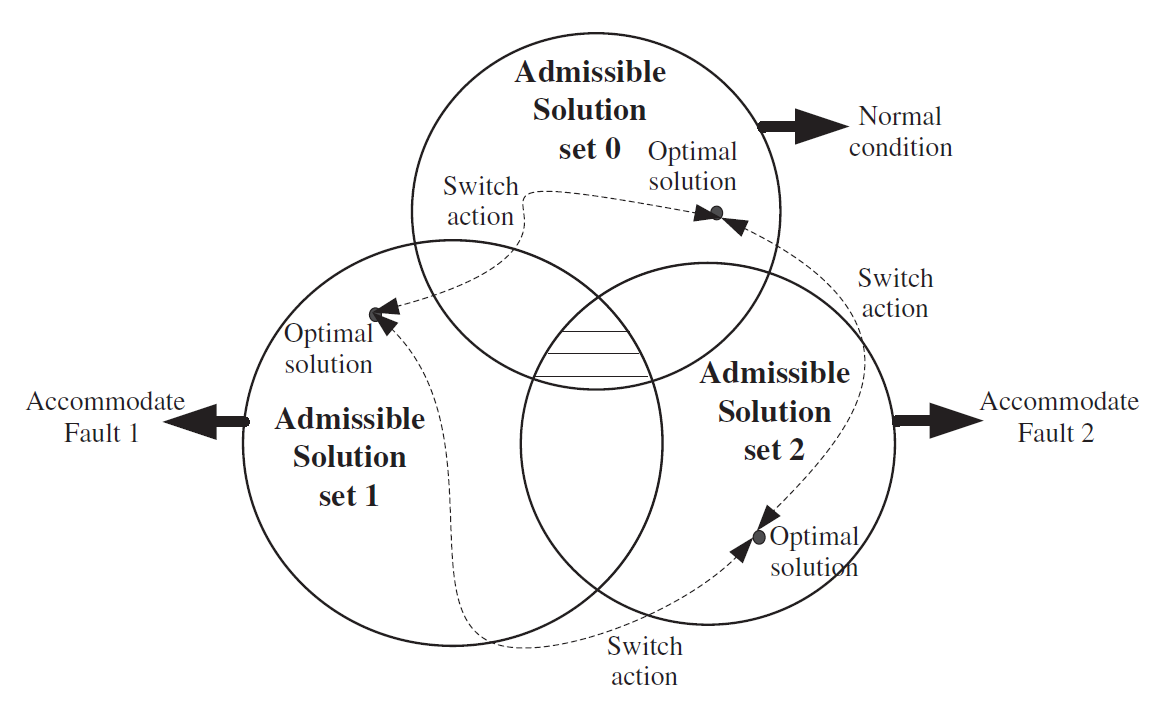
\includegraphics[width = 0.9\textwidth]{figure/admissiblesp.png}
    \bicaption[fig:asp]{可接受的控制空间示意}{可接受的控制空间示意\cite{Jiang201260}}{Fig.}{The acceptable space}
\end{figure}
\begin{figure}[!htp]
    \centering
    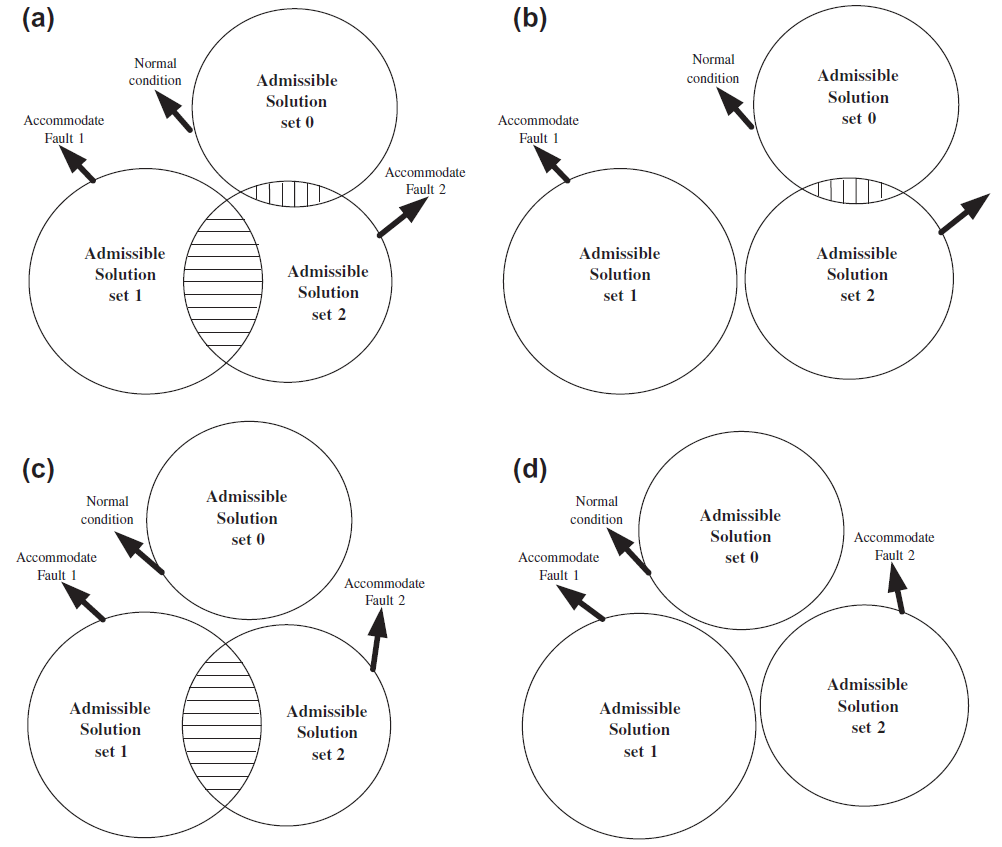
\includegraphics[width = 0.9\textwidth]{figure/aspoverlap.png}
    \bicaption[fig:aspoverlap]{其他控制器空间示意}{其他控制器空间示意\cite{Jiang201260}}{Fig.}{Other controller's space}
\end{figure}

被动容错控制文献中被称为可靠控制(Reliable control)。“可靠”的概念第一次由Siljak于1980年提出\cite{siljak1980},经过Date和Cho等人的发展\cite{70346,4790503},最终在1992年由Robert J. Veillette进行系统地总结\cite{119629},提出了“可靠控制”这一概念。往后,文献中的凡是以被动容错控制思路设计的控制器,都以reliable control呈现。

被动容错控制的设计方法有很多种,在$H_\infty$优化\cite{119629,7850999}、LMI方法\cite{7795198,974340,1236798}、LQ方法\cite{VEILLETTE1995137,847106,866928},滑模控制方法\cite{4160860},模糊系统\cite{7795198,7505963,Zha20173267},动态预补偿结合特征结构配置\cite{Jiang2000Design,ZHAO19981267},去中心化观测器\cite{70346}等方面均有相关研究成果。其中文献\cite{ZHAO19981267}首次给控制器冗余和错误构建了数学模型。另外,根据针对系统错误的不同,被动容错控制还可以分为针对执行机构失效\cite{ZHAO19981267,974340,VEILLETTE1995137,1236798,Tian20101907,Li20132455,7353144,7863042,70346,866928}、时变错误\cite{7850999,CHEN2004349,6064886}和随机错误\cite{7795198,7505963,5540530,Zha20173267}。基于控制器重构的被动容错控制也受到了不少关注\cite{6859271},这一类控制器通过重新分配控制量的方法来使控制器适应多种错误。
国内外也有不少文献对被动容错控制提出了分类方法。国外文献中,Fekih\cite{6859271}用鲁棒控制的分类方法把被动容错控制分为了数量反馈理论法、$H_\infty$范数优化法\cite{4079591}、LQ控制法\cite{Staroswiecki20072070}、$\mu$同步法和变结构方法。国内文献中,王德军\cite{wangdejun2014}、许德智\cite{xudezhi2013}和高志峰\cite{gaozhifeng2011}都将被动容错控制分为可靠镇定、完整性与联立镇定三类方法。肖冰\cite{xiaobing2014}认为在航天器姿态控制中,被动容错控制可以与主动容错控制的控制器重构部分做为一个方向共同研究。他将航天器姿态容错控制方法,分为基于自适应技术(Adaptive)的方法、基于滑模控制的方法和基于控制分配的方法三类,这一点在Yin. S的论文中\cite{7407616}也得到了有力的支撑。

\subsection{故障检测与故障诊断}\label{subsec:fdd}

故障检测(Fault Detection)与故障诊断(Fault Diagnosis)是两个不同的概念。故障检测,一般指系统对是否发生故障进行在线检测;而故障诊断,指的是在检测到故障的基础上,判断故障的类型和严重性。故障检测与诊断是主动容错控制器设计前的必经步骤。目前已经有很多综述文章阐述了故障检测与诊断的研究现状\cite{Venkatasubramanian2003293,6859271,Zhang2008229,7407616,6423903,Marzat2012modelbased,Jiang201260,5282515,Venkatasubramanian2003293,Venkatasubramanian2003A}。其中具体对故障检测的分类也有一些不同。

Inseok Hwang\cite{5282515}在文献中将故障检测分为硬件冗余(Hardware Redundancy)和分析冗余(Analytical Redundancy)两类。而其中硬件冗余主要是设计多传感器来尽可能明确地检测故障,可分为交叉频道监控(Cross channel monitoring, CCM)、残差生成(Residual Generation)和信号处理(Signal Processing)方法;分析冗余主要是用数学模型直接对系统当前状况进行估计,不需要多余的硬件,因此也更高效,分析冗余又可分为定性(Qualitative)方法和定量(Quantitative)方法。 Fekih\cite{6859271}和Hwang\cite{5282515}都认为所有故障检测都由三个步骤构成:残差生成(Residual Generation)、残差评估(Residual Evaluation)和最终判断(Decision Making)。在此基础上,诊断方法可以分为基于模型(Model-Based)的方法和不基于模型(Model-Free)的方法。其中基于模型的方法有模糊、神经网络、专家系统等方法\cite{Patan2008Artificial},不基于模型的方法主要是基于算法和统计的手段。而残差评估则可以分为序列概率检验(Sequential probability ratio test)和通用比例检验(Generalized Likelihood Ratio Test)等统计学上的方法\cite{5282515}。此外,Yin的文献\citen{7407616}中把故障检测分为两大类——基于模型的方法和基于数据的方法。其中基于模型的方法依赖于系统模型,而当模型不准确时,可以使用纯数据方法。

本文的观点与Fekih\cite{6859271}和Hwang\cite{5282515}各有相似之处,认为不论基于模型还是数据,故障检测的思路都是通过设计一个残差函数来对故障进行判断,具体在残差函数的设计思路及依赖上,才有了基于模型、不基于模型或是基于数据的区别。因此,本文故障检测的步骤分为残差生成、残差评估两个步骤。而残差生成作为故障检测的核心部分,又可以分为基于模型的方法和基于数据的方法。
\subsubsection{基于模型的方法}
对于基于模型的方法,文献\citen{Marzat2012modelbased}做了很好的综述。Venkatasubramanian的两篇综述\citen{Venkatasubramanian2003293,Venkatasubramanian2003A}将基于模型的故障检测分为定性方法和定量方法。通常来说,该类故障检测分为残差生成、残差评估两个环节\cite{Marzat2012modelbased},系统框图如图\newref{fig:FDDProcess}所示。在残差生成环节,使用系统的执行器输入和传感器数据来预测系统接下来的行为;然后将预测行为与系统实际行为进行比较。这里介绍几种基于模型的方法,分别是参数估计类方法、状态估计类方法、奇偶校验空间方法、去耦合类方法和闭环方法。
\begin{figure}[htp]
    \centering
    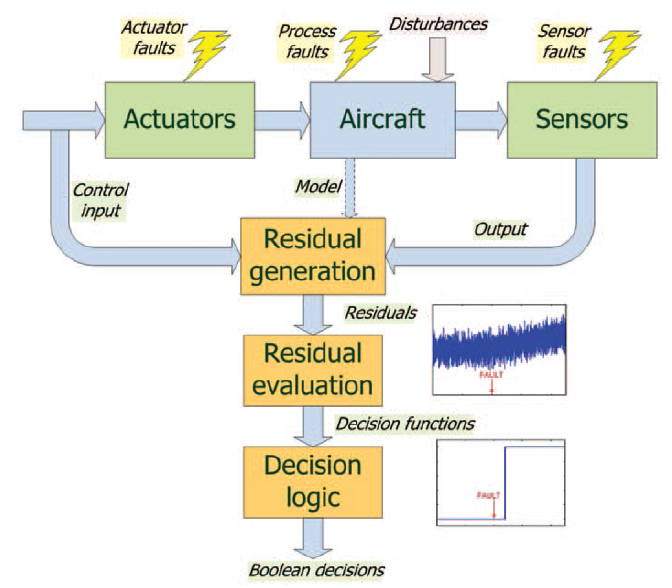
\includegraphics[width = 0.9\textwidth]{FDDProcess.png}
    \bicaption[fig:FDDProcess]{一种典型的故障检测机制}{一种典型的故障检测机制}{Fig.}{A typical fault detection scheme}
\end{figure}

\paragraph*{参数估计类方法}由于系统方程中的参数很可能没有直接的物理意义,而有些能测量到的物理量又不能明显地给出系统是否有错误的判断,参数估计故障诊断方法就是在这种背景下产生的。这类方法的思路是:把系统方程中的参数$\theta$与系统中具有实际物理意义但不能测量到的变量$p_a$(如舵偏角等)建立方程
$$\theta = g_p(p_a)$$
然后首先依据系统观测方程
$$y=h(u,\theta)$$
测量到的$y$对参数$\theta$进行估计,得到$\hat{\theta}$;再通过$p_{a0} = g_p^{-1}(\hat{\theta})$求出可能的$p_{a0}$。最后将得到的$p_{a0}$输入事先设计好的残差函数,与事先设置好的可接受的$p_a$值进行比较。这是一种比较经典的方法,文献多在2000年以前出现\cite{ISERMANN1984387,FRANK1990459,ISERMANN1993815,411478,BLOCH19951709},其中对参数$\hat{\theta}$的辨识也成为了新的研究方向\cite{ISERMANN1993815,411478,BLOCH19951709},涉及到的方法多为最小二乘、卡尔曼滤波等一些最优估计的方法。参数估计的计算强度较大是这类方法的缺点,文献\cite{Villemonteix2009Bayesian}对参数估计提出了一种贝叶斯(Bayesian)优化方法。在残差函数的设计中,也可以设置多个可接受的$p_a$值的集合,详见文献\citen{Kieffer2011Guaranteed,Puig2010Fault}。

\paragraph*{状态估计类方法}状态估计类方法的思路是通过对系统状态的估计与传感器测量的数据做对比,得到系统是否发生错误的判决。通常可以根据对不确定性的处理分为确定性方法、随机方法和有界误差方法\cite{Marzat2012modelbased}。

确定性方法\cite{1098323,ALCORTAGARCIA1997663}不考虑系统的误差和扰动,直接在模型中推导观测误差与错误的关系。Luenberger观测器\cite{1098323}是这种方法第一次被应用到线性系统上。由于非线性系统线性化的时候会产生误差,因此又有了处理非线性系统的扩展Luenberger观测器(Extended
Luenberger Observer, ELO)\cite{Nejjari2008Extended,ZEITZ1987149}。此外,由于非线性系统的复杂性,也有很多种观测器得到了研究,如自适应观测器(Adaptive observers)\cite{878691,Zhang2010290}、高增益观测器(High-gain observers)\cite{Busvelle2002HIGH}、滑模观测器(Sliding Mode Observers)\cite{Edwards2011Sliding,1269645}和基于偏微分方程(partial-differential equation)设计的新型观测器\cite{5717995}。

随机方法中,通常假定系统的噪声扰动服从高斯分布(Gaussian Distribution),在处理线性系统时以卡尔曼滤波器(Kalman Filter)为代表。基于卡尔曼滤波器的容错方法首先在文献\cite{MEHRA1971637}中提到,而后\cite{NIKOUKHAH19941851,539440,willsky1986detection}做了后续延伸工作。处理非线性系统时,有扩展卡尔曼滤波(Extended Kalman Filter, EKF)、无迹卡尔曼滤波(Unscented Kalman Filter, UKF)和粒子滤波(Particle Filter, PF)。扩展卡尔曼滤波通过对非线性系统线性化来使用卡尔曼滤波\cite{CHANG19952861};无迹卡尔曼滤波则不对系统线性化,通过一些系统状态采样点来逼近系统状态的高斯分布\cite{4252507,XIONG2005113}。粒子滤波则可适用于非线性非高斯分布的噪声,它采用蒙特卡洛方法对错误进行建模并估计\cite{1271398,971661}。

有界误差方法不同与上面两种。上面两种都使用了显示的故障模型或概率分布,而有界误差方法使用故障的上界进行处理。这类方法的文献如区间分析法\cite{4547434}和神经-模糊方法\cite{Korbicz2007609}。

\paragraph*{奇偶校验空间法}奇偶空间校验(Parity Space)方法比较容易从直观上理解,是一种解除系统状态和错误之间的耦合,从而方便设计出只跟故障有关的残差函数\cite{patton1991review,GERTLER1995627}的方法。具体来说,对于一个静态线性观测系统:
\begin{equation*}
    \mathbf{y} = \mathbf{Cx} + \mathbf{E_fw_f}
\end{equation*}
其中$\mathbf{w_f}$是系统错误,$\mathbf{y}$是观测变量。此时如果设计一个矩阵$\mathbf{W}$,使得$\mathbf{WC=0}$,那么残差函数$\mathbf{Wy}$就只与系统错误$\mathbf{w_f}$有关了,可以依次设计残差函数。对于动态系统,可以用\citen{Marzat2012modelbased}中提及的方法先把系统化成静态系统的形式。对于非线性系统,则可以用线性化、仿射变换等方式来处理,详见文献\citen{Staroswiecki2001687,shumsky2007redundancy,1024022,948476}。

\paragraph*{去耦合类方法}在故障检测设计残差函数时,经常遇到的一个问题是如何区分系统的正常扰动和意外故障。一个理想的残差函数应该满足\cite{1104419}:1)只对系统错误有响应,对系统状态和扰动无响应;2)在系统没有故障的时候,能够随着时间的推移收敛到0。这里介绍四种去耦合类的方法。

第一种是特征结构分配(Eigenstructure Assignment)的方法\cite{261546}。该方法给系统的输出估计偏差$\mathbf{e_y}$左乘了一个权值矩阵$\mathbf{W}$作为残差函数\cite{261546,RNC:RNC523}。同样的方法也可以用在奇偶校验空间的残差设计中,使得残差对系统扰动不敏感\cite{doi:10.1080/00207179508921908}。

第二种是未知输入观测器(Unknown-Input Observer, UIO)。这种观测器能够在估计系统状态的同时将外部扰动的影响降到最小\cite{jie1996design,1657536,220921}。简单将未知输入观测器的原理说明如下,假设系统如\neweqref{eq:UIO1}所示。
\begin{equation}\label{eq:UIO1}
\begin{cases}
\dot{x} = Ax+Bu+E_dw_d+E_fw_f \\
y = Cx 
\end{cases}
\end{equation}
其中$w_d$代表扰动,$w_f$代表错误。针对该系统的位置输入观测器设计如\neweqref{eq:UIO2}所示
\begin{equation}\label{eq:UIO2}
\begin{cases}
\dot{\hat{x}}=F\hat{x}+TBu+(K_1+K_2)y \\
\mathbf{r} = (I-CH)y-C\hat{x}
\end{cases}
\end{equation}
其中,$\mathbf{r}$为残差函数,$F,T,K_1,K_2,H$都是设计参数,需满足以下条件:
\begin{equation*}
\begin{cases}
(HC-I)E_d=0\\
T = I - HC\\
F= I-HCA-K_1C\\
K_2=FH
\end{cases}
\end{equation*}
只要这样的观测器存在,那么可以用\citen{4101989}中提及的DOS(Dedicated observer scheme)或者GOS(General observer scheme)的方法进行故障检测系统设计。

第三类方法是$H_{\infty}$方法,这种策略适合精确解耦无法达到的情况\cite{doi:10.1080/002071799220704,Henry2005251}。$H_{\infty}$方法的思想是,根据$H_{\infty}$范数设计残差函数,使得错误对其影响最大,并且扰动对其影响最小。运用线性矩阵不等式(Linear Matrix Inequality, LMI)是解决这类问题的标准化方法\cite{Zhong2003543}。

第四类是非线性几何方法。微分几何的方法\cite{928586,Bokor2009113}能够检测是否存在一个只对一种错误敏感的滤波器\cite{Marzat2012modelbased}。微分代数的方法也有文献,如\citen{berdjag:hal-00198435}。此外,还有一种逆向的方法\cite{edelmayer2004input,doi:10.1080/00207170802582215,1102181}。该种方法不同于大多数故障检测方法。大多数故障检测系统都使用估计系统输出与测量到的系统输出作比较或设计残差函数,这种逆向方法使用系统输入与前一时段发送给系统执行器的输入作比较。由于大多数飞行器都装备了惯性测量元件(Inertia Measurement Unit, IMU),针对利用惯性测量元件的故障检测也有相关文献,如\citen{MARZAT2010951,5676073}。

\paragraph*{闭环方法}前面介绍的几种故障检测方法都是未考虑反馈控制的开环检测方法。但事实上控制信息能极大地辅助故障检测。比如设计一个辅助控制器添加到系统本身的输入中\cite{NIEMANN2006587,ASHARI2009192}。文献\citen{ASHARI2009192,4602147}将这种方法应用到无人机上,通过添加一个微小的正弦控制量的方法进行故障检测。但是这种方法需要非常小心,需要保证添加的控制量不会严重干扰系统的稳定性和表现\cite{Niemann2006Active}。

鉴于以上原因,闭环方法需要在控制表现和故障检测能力中做取舍。Jacobson\cite{92987}设计了同时能够控制和故障检测的模型。 相关的多目标优化问题也成为了研究的热点。Henry\cite{Henry2005251}提出了一种对这类问题的建模,并用线性矩阵不等式得到了问题的最优解。Niemann\cite{649678}对闭环故障检测方法的效果与开环方法做了对比。

\subsubsection{基于数据的方法}\label{subsubsec:databased}
当系统模型十分不精确,没有显示表达甚至无法获取的时候,人们对系统的认知途径只能通过测量的方式。通过测量到的数据,加上一定的分析方法,能够最大限度地还原系统的面貌。这时,系统相当于一个黑盒,其历史运行数据是掌握其运行规律的唯一方法。通过数据,不仅可以对系统进行故障诊断,还能进行控制器设计。这一类方法统称基于数据的方法。在1991年,Jackson已经使用多变量统计学进行故障检测。

Yin在基于数据的方法有较多的研究文献\cite{6717991,7394158,7067026,6748057,7297846,7407616}。其中文献\cite{6717991,6748057,7407616}提供了基于数据的故障诊断的文献综述。此外,Qin\cite{Qin2012220}、Marzat\cite{Marzat2012modelbased}、Venkatasubramanian\cite{Venkatasubramanian2003327}都做了对基于数据故障检测方法的综述。其中Qin\cite{Qin2012220}对残差生成、残差判别、故障识别等多个步骤都做了综述。由于残差生成是故障检测的核心步骤,这里介绍几种基于数据的残差生成的方法。几种方法的思路都是给系统的正常状态建模,或者建立一个系统正常状态下的向量空间。如果测量得到的数据偏离了这个空间,那么就说明系统出现了错误。学术界这一类容错的方法有专家系统(Expert System)方法、主成分分析法(Principle Component Analysis, PCA)和模式识别方法等。由于专家系统方法现在应用较少,下面主要介绍主成分分析法和模式识别方法。

\paragraph*{主成分分析法}
主成分分析\cite{jolliffe2002principal}在工程中有非常广泛的应用,适用于能获取到大量历史运行数据的系统。Ding\cite{Ding2010138}对标准主成分分析在故障检测中的应用做了介绍。主成分分析通过对矩阵的奇异值分解,能够得到矩阵行空间或者列空间中对矩阵影响最大的$k$组基,这$k$组基扩展而成的空间就是正常空间范围,如果系统测量到的数值偏离了这个正常空间过多,那么可以判定系统运行出了错误。假定测量的数据是由$m$个传感器测量得到的$\mathbf{x}\in \mathcal{R}^m$。对系统进行$N$次测量后得到的数据是可以表示为$\mathbf{X}=[\mathbf{x_1},\mathbf{x_2},\cdots,\mathbf{x_N}]^T\in \mathcal{R}^{m\times N}$,其中第$k$次测量结果为$\mathbf{x_k}^T$。那么$\mathbf{X}$样本的协方差矩阵为
\begin{equation*}
    \mathbf{S} = \frac{1}{N-1}\mathbf{X}^T\mathbf{X}
\end{equation*}
对$\mathbf{S}$进行对角化,得到
\begin{equation*}
\mathbf{S}=\begin{bmatrix}\mathbf{T}& \tilde{\mathbf{T}}\end{bmatrix}\begin{bmatrix}\Lambda& O\\O&\tilde{\Lambda}\end{bmatrix}\begin{bmatrix}\mathbf{T}& \tilde{\mathbf{T}}\end{bmatrix}^T
\end{equation*}
其中$\mathbf{T}$是$m\times l$维矩阵,$l$是事先选取好的主要成分的维度。那么对于一个新的测量$\mathbf{x}$,它在主要成分和非主要成分空间上的投影分别为
\begin{eqnarray}
\text{主要空间:}\hat{\mathbf{x}} = \mathbf{TT}^T\mathbf{x} \\
\text{非主要空间:}\tilde{\mathbf{x}} = \tilde{\mathbf{T}}\tilde{\mathbf{T}}^T\mathbf{x}
\end{eqnarray}
后续依此可以设计残差函数,如$\tilde{\mathbf{T}}$的范数就是一个在无故障时很小的值。
主成分分析的优点是运算速度快,缺点是要求被测量和变化量是线性关系,这一点也是制约主成分分析精确程度的一个重要因素。在已有文献中,Lee\cite{Lee2004223}用核主成分分析(Kernel Principle Component Analysis)对非线性关系进行了探索。独立成分分析(Independent Component Analysis)也可以解决非线性问题\cite{Li20111015}。此外,主成分分析还有一些别的引申和变种\cite{Luo1999sensor,Harkat2006625,4602224,Misra20021281},包括处理动态系统的动态主成分分析\cite{Luo1999sensor},修正协方差矩阵的鲁棒主成分分析\cite{4602224}和处理固定模型的迭代主成分分析(Recursive PCA)等。主成分分析还有一种很相似的方法,叫偏最小二乘法(Partial Least Squares, PLS),用来处理数据维度大于样本或者数据变量之间耦合程度比较高的情况\cite{Wang2003613,JOEQIN1998503,6873303}。

\paragraph*{模式识别方法}
故障检测的本质其实是一种分类方法,而模式识别则提供了大量基于数据的分类方法。这类方法的思路是,首先给根据自己对系统的先验知识给系统的错误进行分类,并设置好每一类的故障向量空间。具体的分类可以用K-means等\cite{Patton1999}聚类算法实现。如果数据库中只有系统正常运行的数据,可以用单类支持向量机(One-class support vector machine)处理\cite{Mahadevan20091627,Chandola2009Anomaly}。根据使用的工具分类,模式识别方法可以分为使用神经网络、支持向量机等手段的方法。

综述\citen{824819}给出了模式识别的常见方法。最简单的情况是计算两类之间的边界函数$f(x)$,根据$f(x)$的正负来判断向量$x$的归属类别。寻找边界函数的方法有很多,在数据已有的情况下,神经网络是最普遍的一种\cite{897072,Chen2002101}。神经网络在故障检测中的使用也很普遍\cite{Chen2002101,FRANK199767,Markou20032481}。神经网络有两种架构——有监督学习和无监督学习。在有监督学习中\cite{Caruana2006empirical},只要选定了网络的拓扑结构,识别错误的问题就可以化简为估计神经元之间的权值,而这些权值可以由已有的有故障或正常的数据学习而来。在无监督学习中,神经网络也叫自组织网络(Self-organizing Network)。在这种情况下,网络结构是跟着网络输入自适应地变化的,如ART2网络\cite{33}。90年代最流行的有监督学习训练神经网络的方法是方向传播(Back-propagation, BP)法。此外,支持向量机(Support Vector machine, SVM)方法也是一种重要的用于故障检测的分类方法\cite{788640}。支持向量机是一种把数据映射到高维空间并寻找分界的方法;它通过设置一个风险函数并将其最小化的方法,寻找这个界面\cite{vapnik2013nature}。其他关于模式识别故障检测常见的方法详见文献\citen{Ge2004143,Davy20062009,Liu2017401,7813447,Markou20032499}

\subsection{控制器重构}\label{subsec:active}
可重构控制器(Reconfigurable controller)指的是能够自动根据在线信息重新生成控制信息的控制器。本文讨论的可重构控制器特指基于故障检测的可重构控制器。在主动容错控制中,当故障检测系统成功检测并识别出故障之后,系统会针对已发生的错误种类,实时生成能够让系统继续保持稳定的控制器。除了基于故障检测之外,可重构控制器还有基于其他信息的类型,如迭代学习控制\cite{1636313}(Iterative Learning Control, ILC),这一类不在本文的讨论范围之列。

控制器重构的方法也是一个重要的研究热点,因此也有一些不同的分类。Hwang\cite{5282515}将控制器重构分为多模型(Multi-model)方法和自适应(Adaptive)方法;Zhang\cite{Zhang2008229}对控制器重构做了多种分类,详见图\newref{fig:recclass};Yin\cite{7407616}将控制器重构分为自适应方法、滑模(Sliding mode)方法和基于控制分配(Control allocation)的方法;Fekih\cite{6859271}将控制器重构分为两类——事先计算好的方法和实时计算的方法。
\begin{figure}
    \centering
    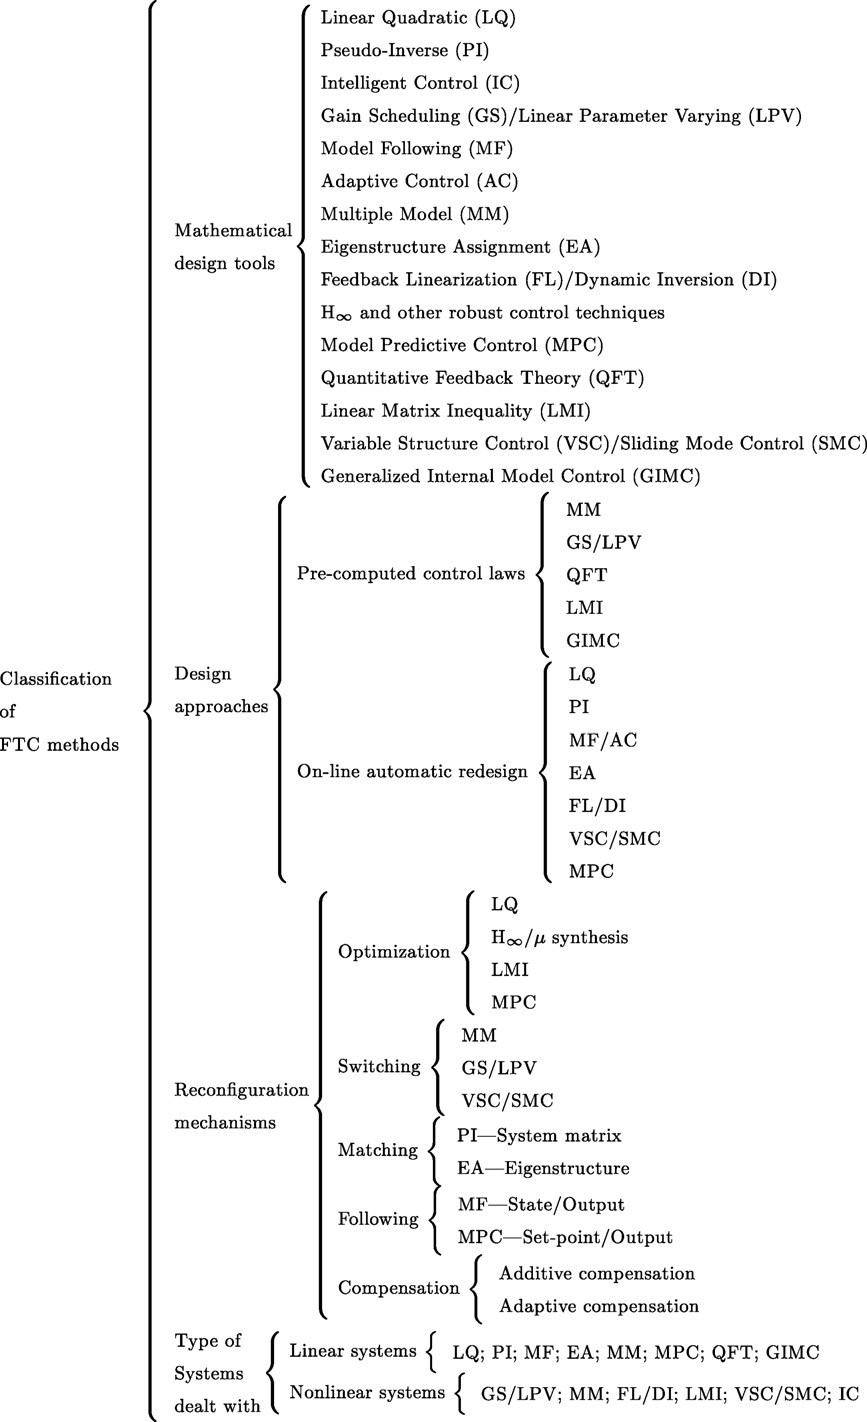
\includegraphics{Reconclass.jpg}
    \bicaption[fig:recclass]{控制器重构方法的分类}{控制器重构方法的分类\cite{Zhang2008229}}{Fig.}{The classification of controller reconfiguration methods}
\end{figure}
结合以上不同的分类,这里主要介绍三类控制器重构的方法——多模型方法、自适应方法和滑模方法。事实上,图\newref{fig:recclass}中提到的10多种方法之间也都有混合与交叉,很少有一种重构方法只依赖一种模型\cite{Zhang2008229}。

\paragraph*{多模型方法}
多模型方法的思路是,用平行的$N$个已知参数的模型来预测系统在不同错误情形下的下一步状态有哪些可能,然后根据测量得到的状态选择一个预测最准确的模型作为参考模型,预测的工具通常使用卡尔曼滤波器。事先给每个模型设计好控制器,一旦确定了错误种类,就立即将控制器切换成该种模型对应的控制器。这种故障重构机制没有在线计算的过程,控制器都是提前设计好的,模型也是提前根据不同错误类型构建的。因此理论上有多少种模型就能够处理多少种错误。

这一类方法主要有两种\cite{5282515}:多模型自适应估计(Multiple model adaptive estimation, MMAE)\cite{81428,70412}与交互多模型(Interacting multiple model, IMM)\cite{976961,827910},其中后者是为了解决系统参数变化的问题而提出的。此外,在飞行器的容错控制领域还有其他基于多模型方法的容错设计,如文献\cite{827910,786187,JUNG2005115}。

\paragraph*{自适应方法}
自适应控制器重构方法\cite{1709933,6670789,7353144}是最为常见的控制器重构策略。Boskovic\cite{703075}对控制输入变量大于控制输出变量的控制器提出了一种自适应控制器重组的方法,在多执行机构卡顿的情况,并且控制器不知道错误信息的情况下能够保持系统稳定。Chen\cite{989090}提出了一种处理输入信号卡顿的控制方法,并给出了针对执行器故障的补偿条件。Zuo\cite{6945860}针对线性和非线性但满足Lipschitz条件的多智能体系统提出了自适应容错控制。自适应方法也通常与神经网络\cite{6060930,Lin2017}、滑模控制\cite{6060930,7506323}、反演(Backstepping)\cite{Li2016177,Jiang201057}、模糊控制\cite{Zou201110}等其他方法结合使用。

\section{当前研究存在的问题}
当前针对容错控制的研究虽然有很多,但是由于平流层飞艇的特殊性,一般的容错控制方案并不能满足其需要。具体来说,平流层飞艇主要有如下特殊之处:
\begin{enumerate}
  \item 平流层飞艇由于内部充气,并工作在空气稀薄的环境下,因此昼夜温差巨大,所以其模型中的惯性矩阵和气动系数在不同时间将会急剧变化。
  \item 平流层飞艇受限于其载重限制,因此执行机构通常远远不能满足控制需要,饱和现象经常出现,需要在容错控制器的设计中考虑到。
  \item 平流层飞艇通常需要长时间工作在临近空间的恶劣环境下\cite{fenggui2013},因此其执行机构非常容易出现卡顿、失效等故障。一般的应对执行机构卡顿的方法。
  \item 平流层飞艇容易受到风的干扰,除此之外还会受到各种不稳定的气流,造成实际故障无法准确跟踪。
  \item 传统的Super-Twisting观测器应用于平流层飞艇进行故障重构的时候,其收敛速度非常缓慢,不能应用于实际中。
\end{enumerate}
因此,在实际中,平流层飞艇会遇到一些以前的研究没有考虑到的问题。所以针对平流层飞艇的研究不能完全采用一般的针对非线性系统的容错控制研究方案,需要单独针对平流层飞艇的模型设计控制方案或者故障重构方案。

\section{本课题创新点}
本课题主要针对浮空器经常出现的一些不确定性、故障和控制难点进行了容错控制器设计。本文的研究内容和创新点主要分为三个部分,分别是:
\begin{enumerate}
    \item 针对平流层飞艇的惯性矩阵和气动矩阵的不确定性,设计了一种自适应滑模容错控制方案。
    \item 针对平流层飞艇的惯性矩阵、气动矩阵的不确定性以及执行机构的效率损失和输出偏移等故障,设计了一种自适应滑模容错控制方案。
    \item 针对Super-Twisting观测器应用于平流层飞艇收敛速度慢的问题,提出了一种改进的Super-twisting观测器,增加了使其收敛速度可调节的参数,并证明了新观测器的稳定性。
\end{enumerate}
